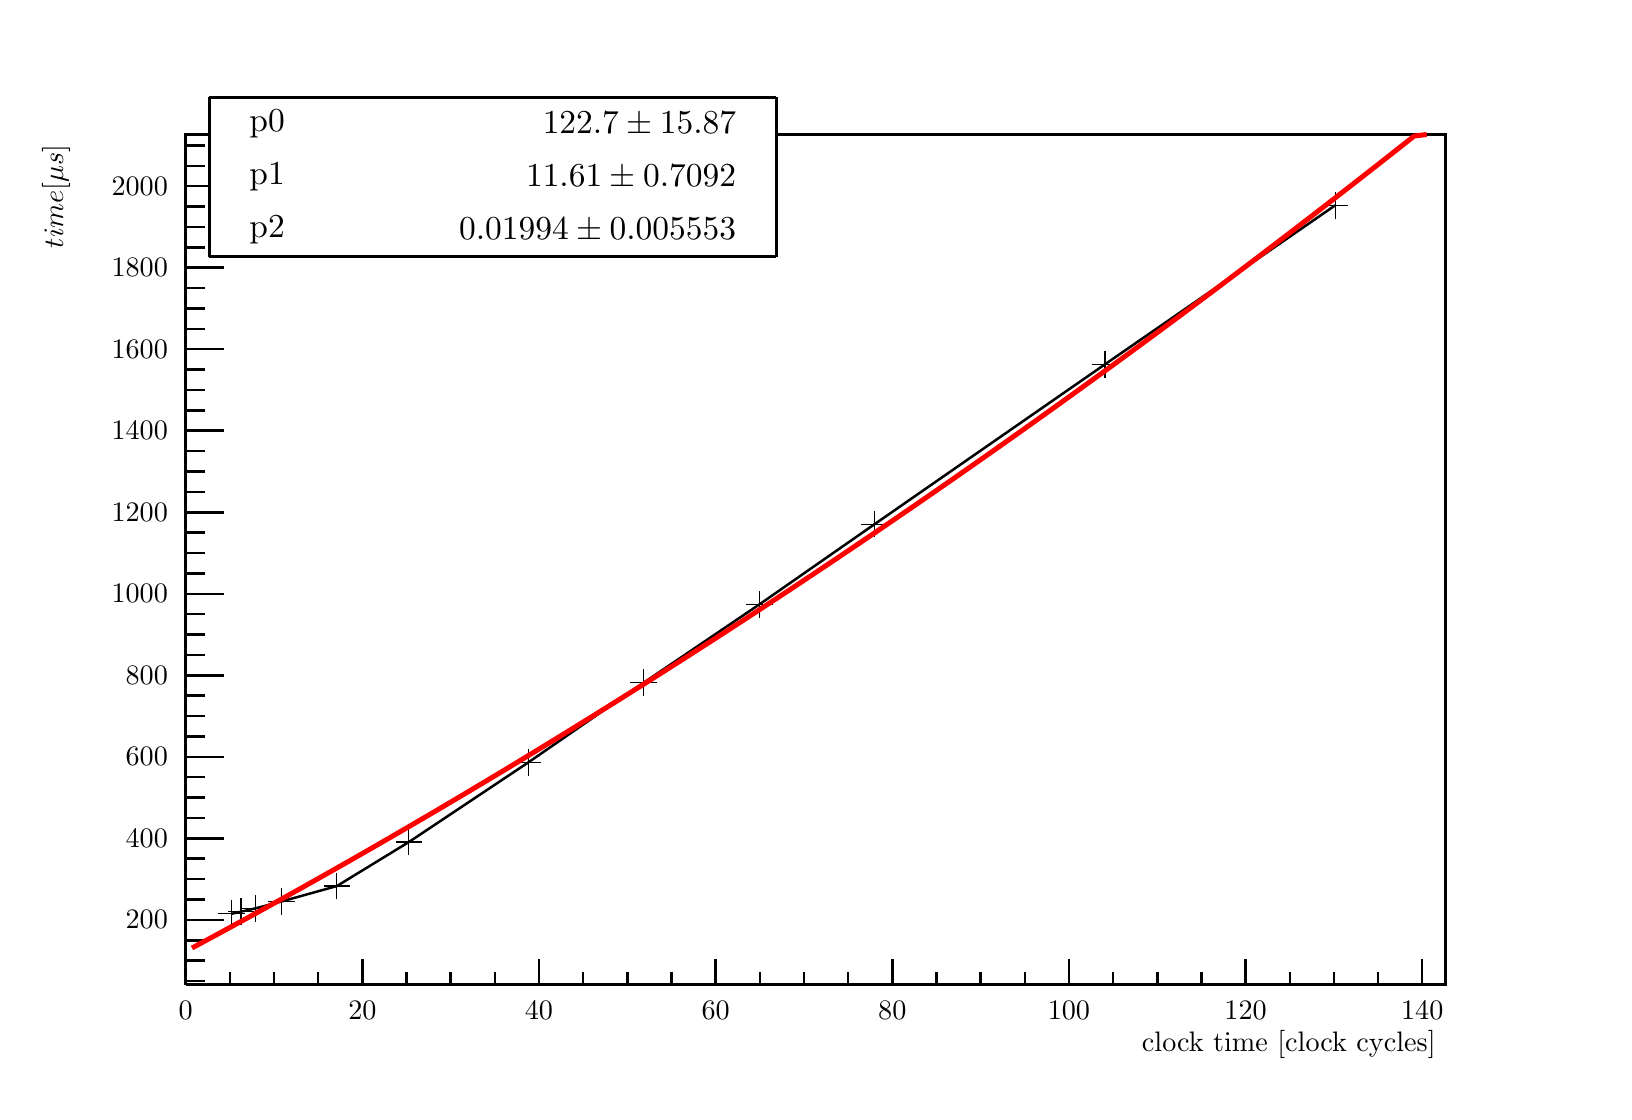
\begin{tikzpicture}
\pgfdeclareplotmark{cross} {
\pgfpathmoveto{\pgfpoint{-0.3\pgfplotmarksize}{\pgfplotmarksize}}
\pgfpathlineto{\pgfpoint{+0.3\pgfplotmarksize}{\pgfplotmarksize}}
\pgfpathlineto{\pgfpoint{+0.3\pgfplotmarksize}{0.3\pgfplotmarksize}}
\pgfpathlineto{\pgfpoint{+1\pgfplotmarksize}{0.3\pgfplotmarksize}}
\pgfpathlineto{\pgfpoint{+1\pgfplotmarksize}{-0.3\pgfplotmarksize}}
\pgfpathlineto{\pgfpoint{+0.3\pgfplotmarksize}{-0.3\pgfplotmarksize}}
\pgfpathlineto{\pgfpoint{+0.3\pgfplotmarksize}{-1.\pgfplotmarksize}}
\pgfpathlineto{\pgfpoint{-0.3\pgfplotmarksize}{-1.\pgfplotmarksize}}
\pgfpathlineto{\pgfpoint{-0.3\pgfplotmarksize}{-0.3\pgfplotmarksize}}
\pgfpathlineto{\pgfpoint{-1.\pgfplotmarksize}{-0.3\pgfplotmarksize}}
\pgfpathlineto{\pgfpoint{-1.\pgfplotmarksize}{0.3\pgfplotmarksize}}
\pgfpathlineto{\pgfpoint{-0.3\pgfplotmarksize}{0.3\pgfplotmarksize}}
\pgfpathclose
\pgfusepathqstroke
}
\pgfdeclareplotmark{cross*} {
\pgfpathmoveto{\pgfpoint{-0.3\pgfplotmarksize}{\pgfplotmarksize}}
\pgfpathlineto{\pgfpoint{+0.3\pgfplotmarksize}{\pgfplotmarksize}}
\pgfpathlineto{\pgfpoint{+0.3\pgfplotmarksize}{0.3\pgfplotmarksize}}
\pgfpathlineto{\pgfpoint{+1\pgfplotmarksize}{0.3\pgfplotmarksize}}
\pgfpathlineto{\pgfpoint{+1\pgfplotmarksize}{-0.3\pgfplotmarksize}}
\pgfpathlineto{\pgfpoint{+0.3\pgfplotmarksize}{-0.3\pgfplotmarksize}}
\pgfpathlineto{\pgfpoint{+0.3\pgfplotmarksize}{-1.\pgfplotmarksize}}
\pgfpathlineto{\pgfpoint{-0.3\pgfplotmarksize}{-1.\pgfplotmarksize}}
\pgfpathlineto{\pgfpoint{-0.3\pgfplotmarksize}{-0.3\pgfplotmarksize}}
\pgfpathlineto{\pgfpoint{-1.\pgfplotmarksize}{-0.3\pgfplotmarksize}}
\pgfpathlineto{\pgfpoint{-1.\pgfplotmarksize}{0.3\pgfplotmarksize}}
\pgfpathlineto{\pgfpoint{-0.3\pgfplotmarksize}{0.3\pgfplotmarksize}}
\pgfpathclose
\pgfusepathqfillstroke
}
\pgfdeclareplotmark{newstar} {
\pgfpathmoveto{\pgfqpoint{0pt}{\pgfplotmarksize}}
\pgfpathlineto{\pgfqpointpolar{44}{0.5\pgfplotmarksize}}
\pgfpathlineto{\pgfqpointpolar{18}{\pgfplotmarksize}}
\pgfpathlineto{\pgfqpointpolar{-20}{0.5\pgfplotmarksize}}
\pgfpathlineto{\pgfqpointpolar{-54}{\pgfplotmarksize}}
\pgfpathlineto{\pgfqpointpolar{-90}{0.5\pgfplotmarksize}}
\pgfpathlineto{\pgfqpointpolar{234}{\pgfplotmarksize}}
\pgfpathlineto{\pgfqpointpolar{198}{0.5\pgfplotmarksize}}
\pgfpathlineto{\pgfqpointpolar{162}{\pgfplotmarksize}}
\pgfpathlineto{\pgfqpointpolar{134}{0.5\pgfplotmarksize}}
\pgfpathclose
\pgfusepathqstroke
}
\pgfdeclareplotmark{newstar*} {
\pgfpathmoveto{\pgfqpoint{0pt}{\pgfplotmarksize}}
\pgfpathlineto{\pgfqpointpolar{44}{0.5\pgfplotmarksize}}
\pgfpathlineto{\pgfqpointpolar{18}{\pgfplotmarksize}}
\pgfpathlineto{\pgfqpointpolar{-20}{0.5\pgfplotmarksize}}
\pgfpathlineto{\pgfqpointpolar{-54}{\pgfplotmarksize}}
\pgfpathlineto{\pgfqpointpolar{-90}{0.5\pgfplotmarksize}}
\pgfpathlineto{\pgfqpointpolar{234}{\pgfplotmarksize}}
\pgfpathlineto{\pgfqpointpolar{198}{0.5\pgfplotmarksize}}
\pgfpathlineto{\pgfqpointpolar{162}{\pgfplotmarksize}}
\pgfpathlineto{\pgfqpointpolar{134}{0.5\pgfplotmarksize}}
\pgfpathclose
\pgfusepathqfillstroke
}
\definecolor{c}{rgb}{1,1,1};
\draw [color=c, fill=c] (0,0) rectangle (20,13.4957);
\draw [color=c, fill=c] (2,1.34957) rectangle (18,12.1461);
\definecolor{c}{rgb}{0,0,0};
\draw [c,line width=0.9] (2,1.34957) -- (2,12.1461) -- (18,12.1461) -- (18,1.34957) -- (2,1.34957);
\definecolor{c}{rgb}{1,1,1};
\draw [color=c, fill=c] (2,1.34957) rectangle (18,12.1461);
\definecolor{c}{rgb}{0,0,0};
\draw [c,line width=0.9] (2,1.34957) -- (2,12.1461) -- (18,12.1461) -- (18,1.34957) -- (2,1.34957);
\draw [c,line width=0.9] (2,1.34957) -- (18,1.34957);
\draw [c,line width=0.9] (2,1.67347) -- (2,1.34957);
\draw [c,line width=0.9] (2.56085,1.51152) -- (2.56085,1.34957);
\draw [c,line width=0.9] (3.12169,1.51152) -- (3.12169,1.34957);
\draw [c,line width=0.9] (3.68254,1.51152) -- (3.68254,1.34957);
\draw [c,line width=0.9] (4.24339,1.67347) -- (4.24339,1.34957);
\draw [c,line width=0.9] (4.80423,1.51152) -- (4.80423,1.34957);
\draw [c,line width=0.9] (5.36508,1.51152) -- (5.36508,1.34957);
\draw [c,line width=0.9] (5.92593,1.51152) -- (5.92593,1.34957);
\draw [c,line width=0.9] (6.48678,1.67347) -- (6.48678,1.34957);
\draw [c,line width=0.9] (7.04762,1.51152) -- (7.04762,1.34957);
\draw [c,line width=0.9] (7.60847,1.51152) -- (7.60847,1.34957);
\draw [c,line width=0.9] (8.16932,1.51152) -- (8.16932,1.34957);
\draw [c,line width=0.9] (8.73016,1.67347) -- (8.73016,1.34957);
\draw [c,line width=0.9] (9.29101,1.51152) -- (9.29101,1.34957);
\draw [c,line width=0.9] (9.85186,1.51152) -- (9.85186,1.34957);
\draw [c,line width=0.9] (10.4127,1.51152) -- (10.4127,1.34957);
\draw [c,line width=0.9] (10.9736,1.67347) -- (10.9736,1.34957);
\draw [c,line width=0.9] (11.5344,1.51152) -- (11.5344,1.34957);
\draw [c,line width=0.9] (12.0952,1.51152) -- (12.0952,1.34957);
\draw [c,line width=0.9] (12.6561,1.51152) -- (12.6561,1.34957);
\draw [c,line width=0.9] (13.2169,1.67347) -- (13.2169,1.34957);
\draw [c,line width=0.9] (13.7778,1.51152) -- (13.7778,1.34957);
\draw [c,line width=0.9] (14.3386,1.51152) -- (14.3386,1.34957);
\draw [c,line width=0.9] (14.8995,1.51152) -- (14.8995,1.34957);
\draw [c,line width=0.9] (15.4603,1.67347) -- (15.4603,1.34957);
\draw [c,line width=0.9] (16.0212,1.51152) -- (16.0212,1.34957);
\draw [c,line width=0.9] (16.582,1.51152) -- (16.582,1.34957);
\draw [c,line width=0.9] (17.1429,1.51152) -- (17.1429,1.34957);
\draw [c,line width=0.9] (17.7037,1.67347) -- (17.7037,1.34957);
\draw [c,line width=0.9] (17.7037,1.67347) -- (17.7037,1.34957);
\draw [anchor=base] (2,0.904212) node[scale=1.01821, color=c, rotate=0]{0};
\draw [anchor=base] (4.24339,0.904212) node[scale=1.01821, color=c, rotate=0]{20};
\draw [anchor=base] (6.48678,0.904212) node[scale=1.01821, color=c, rotate=0]{40};
\draw [anchor=base] (8.73016,0.904212) node[scale=1.01821, color=c, rotate=0]{60};
\draw [anchor=base] (10.9736,0.904212) node[scale=1.01821, color=c, rotate=0]{80};
\draw [anchor=base] (13.2169,0.904212) node[scale=1.01821, color=c, rotate=0]{100};
\draw [anchor=base] (15.4603,0.904212) node[scale=1.01821, color=c, rotate=0]{120};
\draw [anchor=base] (17.7037,0.904212) node[scale=1.01821, color=c, rotate=0]{140};
\draw [anchor= east] (18,0.593811) node[scale=1.01821, color=c, rotate=0]{clock time [clock cycles]};
\draw [c,line width=0.9] (2,1.34957) -- (2,12.1461);
\draw [c,line width=0.9] (2.48,2.17163) -- (2,2.17163);
\draw [c,line width=0.9] (2.24,2.43047) -- (2,2.43047);
\draw [c,line width=0.9] (2.24,2.6893) -- (2,2.6893);
\draw [c,line width=0.9] (2.24,2.94814) -- (2,2.94814);
\draw [c,line width=0.9] (2.48,3.20698) -- (2,3.20698);
\draw [c,line width=0.9] (2.24,3.46581) -- (2,3.46581);
\draw [c,line width=0.9] (2.24,3.72465) -- (2,3.72465);
\draw [c,line width=0.9] (2.24,3.98348) -- (2,3.98348);
\draw [c,line width=0.9] (2.48,4.24232) -- (2,4.24232);
\draw [c,line width=0.9] (2.24,4.50116) -- (2,4.50116);
\draw [c,line width=0.9] (2.24,4.75999) -- (2,4.75999);
\draw [c,line width=0.9] (2.24,5.01883) -- (2,5.01883);
\draw [c,line width=0.9] (2.48,5.27766) -- (2,5.27766);
\draw [c,line width=0.9] (2.24,5.5365) -- (2,5.5365);
\draw [c,line width=0.9] (2.24,5.79533) -- (2,5.79533);
\draw [c,line width=0.9] (2.24,6.05417) -- (2,6.05417);
\draw [c,line width=0.9] (2.48,6.31301) -- (2,6.31301);
\draw [c,line width=0.9] (2.24,6.57184) -- (2,6.57184);
\draw [c,line width=0.9] (2.24,6.83068) -- (2,6.83068);
\draw [c,line width=0.9] (2.24,7.08951) -- (2,7.08951);
\draw [c,line width=0.9] (2.48,7.34835) -- (2,7.34835);
\draw [c,line width=0.9] (2.24,7.60719) -- (2,7.60719);
\draw [c,line width=0.9] (2.24,7.86602) -- (2,7.86602);
\draw [c,line width=0.9] (2.24,8.12486) -- (2,8.12486);
\draw [c,line width=0.9] (2.48,8.38369) -- (2,8.38369);
\draw [c,line width=0.9] (2.24,8.64253) -- (2,8.64253);
\draw [c,line width=0.9] (2.24,8.90137) -- (2,8.90137);
\draw [c,line width=0.9] (2.24,9.1602) -- (2,9.1602);
\draw [c,line width=0.9] (2.48,9.41904) -- (2,9.41904);
\draw [c,line width=0.9] (2.24,9.67787) -- (2,9.67787);
\draw [c,line width=0.9] (2.24,9.93671) -- (2,9.93671);
\draw [c,line width=0.9] (2.24,10.1955) -- (2,10.1955);
\draw [c,line width=0.9] (2.48,10.4544) -- (2,10.4544);
\draw [c,line width=0.9] (2.24,10.7132) -- (2,10.7132);
\draw [c,line width=0.9] (2.24,10.9721) -- (2,10.9721);
\draw [c,line width=0.9] (2.24,11.2309) -- (2,11.2309);
\draw [c,line width=0.9] (2.48,11.4897) -- (2,11.4897);
\draw [c,line width=0.9] (2.48,2.17163) -- (2,2.17163);
\draw [c,line width=0.9] (2.24,1.9128) -- (2,1.9128);
\draw [c,line width=0.9] (2.24,1.65396) -- (2,1.65396);
\draw [c,line width=0.9] (2.24,1.39513) -- (2,1.39513);
\draw [c,line width=0.9] (2.48,11.4897) -- (2,11.4897);
\draw [c,line width=0.9] (2.24,11.7486) -- (2,11.7486);
\draw [c,line width=0.9] (2.24,12.0074) -- (2,12.0074);
\draw [anchor= east] (1.9,2.17163) node[scale=1.01821, color=c, rotate=0]{200};
\draw [anchor= east] (1.9,3.20698) node[scale=1.01821, color=c, rotate=0]{400};
\draw [anchor= east] (1.9,4.24232) node[scale=1.01821, color=c, rotate=0]{600};
\draw [anchor= east] (1.9,5.27766) node[scale=1.01821, color=c, rotate=0]{800};
\draw [anchor= east] (1.9,6.31301) node[scale=1.01821, color=c, rotate=0]{1000};
\draw [anchor= east] (1.9,7.34835) node[scale=1.01821, color=c, rotate=0]{1200};
\draw [anchor= east] (1.9,8.38369) node[scale=1.01821, color=c, rotate=0]{1400};
\draw [anchor= east] (1.9,9.41904) node[scale=1.01821, color=c, rotate=0]{1600};
\draw [anchor= east] (1.9,10.4544) node[scale=1.01821, color=c, rotate=0]{1800};
\draw [anchor= east] (1.9,11.4897) node[scale=1.01821, color=c, rotate=0]{2000};
\draw [anchor= east] (0.354441,12.1461) node[scale=1.01821, color=c, rotate=90]{$time [\mu s]$};
\draw [c,line width=0.9] (2.58114,2.24928) -- (2.70167,2.27517) -- (2.88067,2.31658) -- (3.21335,2.40459) -- (3.91984,2.6013) -- (4.83385,3.16039) -- (6.34862,4.16985) -- (7.81717,5.18448) -- (9.28622,6.17841) -- (10.7503,7.19823) -- (13.6753,9.2275)
 -- (16.5983,11.2464);
\foreach \P in {(2.58114,2.24928), (2.70167,2.27517), (2.88067,2.31658), (3.21335,2.40459), (3.91984,2.6013), (4.83385,3.16039), (6.34862,4.16985), (7.81717,5.18448), (9.28622,6.17841), (10.7503,7.19823), (13.6753,9.2275),
 (16.5983,11.2464)}{\draw[mark options={color=c,fill=c},mark size=4.804805pt,mark=+] plot coordinates {\P};}
\definecolor{c}{rgb}{1,0,0};
\draw [c,line width=1.8] (2.08,1.81453) -- (2.24,1.90067) -- (2.4,1.98722) -- (2.56,2.0742) -- (2.72,2.16159) -- (2.88,2.24941) -- (3.04,2.33764) -- (3.2,2.4263) -- (3.36,2.51537) -- (3.52,2.60487) -- (3.68,2.69478) -- (3.84,2.78512) -- (4,2.87587)
 -- (4.16,2.96705) -- (4.32,3.05865) -- (4.48,3.15066) -- (4.64,3.2431) -- (4.8,3.33595) -- (4.96,3.42923) -- (5.12,3.52292) -- (5.28,3.61704) -- (5.44,3.71158) -- (5.6,3.80653) -- (5.76,3.90191) -- (5.92,3.99771) -- (6.08,4.09392) -- (6.24,4.19056)
 -- (6.4,4.28762) -- (6.56,4.38509) -- (6.72,4.48299) -- (6.88,4.58131) -- (7.04,4.68004) -- (7.2,4.7792) -- (7.36,4.87878) -- (7.52,4.97878) -- (7.68,5.07919) -- (7.84,5.18003) -- (8,5.28129) -- (8.16,5.38297) -- (8.32,5.48506) -- (8.48,5.58758) --
 (8.64,5.69052) -- (8.8,5.79388) -- (8.96,5.89766) -- (9.12,6.00185) -- (9.28,6.10647) -- (9.44,6.21151) -- (9.6,6.31697) -- (9.76,6.42285) -- (9.92,6.52915);
\draw [c,line width=1.8] (9.92,6.52915) -- (10.08,6.63586) -- (10.24,6.743) -- (10.4,6.85056) -- (10.56,6.95854) -- (10.72,7.06694) -- (10.88,7.17576) -- (11.04,7.285) -- (11.2,7.39466) -- (11.36,7.50474) -- (11.52,7.61524) -- (11.68,7.72616) --
 (11.84,7.8375) -- (12,7.94926) -- (12.16,8.06144) -- (12.32,8.17404) -- (12.48,8.28706) -- (12.64,8.4005) -- (12.8,8.51436) -- (12.96,8.62864) -- (13.12,8.74334) -- (13.28,8.85846) -- (13.44,8.974) -- (13.6,9.08996) -- (13.76,9.20634) --
 (13.92,9.32314) -- (14.08,9.44036) -- (14.24,9.558) -- (14.4,9.67606) -- (14.56,9.79454) -- (14.72,9.91344) -- (14.88,10.0328) -- (15.04,10.1525) -- (15.2,10.2727) -- (15.36,10.3933) -- (15.52,10.5143) -- (15.68,10.6357) -- (15.84,10.7575) --
 (16,10.8798) -- (16.16,11.0025) -- (16.32,11.1256) -- (16.48,11.2491) -- (16.64,11.373) -- (16.8,11.4974) -- (16.96,11.6222) -- (17.12,11.7474) -- (17.28,11.873) -- (17.44,11.999) -- (17.6,12.1255) -- (17.76,12.1461);
\definecolor{c}{rgb}{1,1,1};
\draw [color=c, fill=c] (2.3,10.5941) rectangle (9.5,12.6185);
\definecolor{c}{rgb}{0,0,0};
\draw [c,line width=0.9] (2.3,10.5941) -- (9.5,10.5941);
\draw [c,line width=0.9] (9.5,10.5941) -- (9.5,12.6185);
\draw [c,line width=0.9] (9.5,12.6185) -- (2.3,12.6185);
\draw [c,line width=0.9] (2.3,12.6185) -- (2.3,10.5941);
\draw [anchor= west] (2.66,12.2811) node[scale=1.20912, color=c, rotate=0]{p0       };
\draw [anchor= east] (9.14,12.2811) node[scale=1.20912, color=c, rotate=0]{$ 122.7 \pm 15.87$};
\draw [anchor= west] (2.66,11.6063) node[scale=1.20912, color=c, rotate=0]{p1       };
\draw [anchor= east] (9.14,11.6063) node[scale=1.20912, color=c, rotate=0]{$ 11.61 \pm 0.7092$};
\draw [anchor= west] (2.66,10.9315) node[scale=1.20912, color=c, rotate=0]{p2       };
\draw [anchor= east] (9.14,10.9315) node[scale=1.20912, color=c, rotate=0]{$ 0.01994 \pm 0.005553$};
\definecolor{c}{rgb}{1,1,1};
\draw [color=c, fill=c] (2.3,10.5941) rectangle (9.5,12.6185);
\definecolor{c}{rgb}{0,0,0};
\draw [c,line width=0.9] (2.3,10.5941) -- (9.5,10.5941);
\draw [c,line width=0.9] (9.5,10.5941) -- (9.5,12.6185);
\draw [c,line width=0.9] (9.5,12.6185) -- (2.3,12.6185);
\draw [c,line width=0.9] (2.3,12.6185) -- (2.3,10.5941);
\draw [anchor= west] (2.66,12.2811) node[scale=1.20912, color=c, rotate=0]{p0       };
\draw [anchor= east] (9.14,12.2811) node[scale=1.20912, color=c, rotate=0]{$ 122.7 \pm 15.87$};
\draw [anchor= west] (2.66,11.6063) node[scale=1.20912, color=c, rotate=0]{p1       };
\draw [anchor= east] (9.14,11.6063) node[scale=1.20912, color=c, rotate=0]{$ 11.61 \pm 0.7092$};
\draw [anchor= west] (2.66,10.9315) node[scale=1.20912, color=c, rotate=0]{p2       };
\draw [anchor= east] (9.14,10.9315) node[scale=1.20912, color=c, rotate=0]{$ 0.01994 \pm 0.005553$};
\end{tikzpicture}
